\documentclass[tikz, border=1mm]{standalone}

\newcommand{\arst}{0.5}

\begin{document}
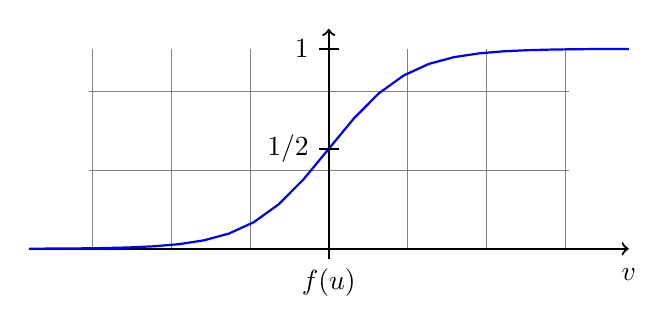
\begin{tikzpicture}[x=1in, y=1in, inner sep=0in, outer sep=0in, domain=-1.5:1.5]

  \draw[very thin,color=gray] (-1.2,0) grid (1.2,1);

  \draw[->, thick] (0,0) -- (0,1.1);
  \draw[->, thick] (-1.5,0) -- (1.5,0) node[anchor=north, outer sep=0.1in] {$v$};

  \draw[thick, blue]    plot (\x,{1/(1 + exp(-\x * 5))});

  \draw[thick, black] (0.05, 0.5) -- (-0.05, 0.5) node[anchor=east, outer sep=0.05in] {1/2};
  \draw[thick, black] (0.05, 1) -- (-0.05, 1) node[anchor=east, outer sep=0.05in] {1};
  \draw[thick, black] (0, 0) -- (0, -0.05) node[anchor=north, outer sep=0.05in] {$f(u)$};

\end{tikzpicture}
\end{document}
